\documentclass[10pt,twocolumn]{article}
\usepackage[margin=0.75in]{geometry}
\usepackage{amsmath,amssymb}
\usepackage{graphicx}
\usepackage{booktabs}
\usepackage{multirow}
\usepackage[numbers,sort&compress]{natbib}
\usepackage{xcolor}
\usepackage[colorlinks=true,linkcolor=black,citecolor=black,urlcolor=blue!50!black]{hyperref}
\usepackage{microtype}
\graphicspath{{../figures/}}
\setlength{\columnsep}{0.25in}

\title{\textbf{FlyArm: A Frozen Whole-CNS Fruit-Fly Connectome\\as the Controller of a Robot Arm}\\[4pt]
\large Technical report}
\author{Yusen Xie\\\small\url{https://github.com/yusenthebot/FlyArm}}
\date{September 2026}

\begin{document}
\maketitle

\begin{abstract}
We use the complete connectome of the adult male \emph{Drosophila} central nervous system (MaleCNS v1.0: 166,700 neurons, 10.5 million connections) as the controller of a simulated Franka arm and never train it.
Only the interface is trained: a sensory encoder that writes currents into the 1,846 ascending neurons and a linear decoder that reads the 1,314 descending and 708 VNC motor neurons into the action; every signal from observation to action passes through three steps of a rate model on the measured wiring per control step.
With imitation followed by PPO with a demonstration term, this controller solves all four tasks of D4RL FrankaKitchen in 50 of 50 test episodes of the official environment, including starts it was never trained on.
On a new articulated multi-step manipulation benchmark (drawers, a lidded cabinet with a shelf, a bin, stacking; tasks of 3 to 8 subgoals over up to 2,600 control steps), skill-level DAgger followed by PPO that also trains the encoder through one step of the frozen connectome reaches 76.3\% full-task success on held-in test episodes and 82.6\% with objects never seen in training, against 63.4\% and 64.7\% for imitation alone, without being told which motor phase of a skill it is in.
Held-out furniture and task orders remain hard (36.6\% and 26.6\%).
We describe the method, the benchmark, what did and did not work, and the controls that are still to run: this report shows that a frozen whole-CNS connectome can be trained to control the arm, not that its wiring is what makes this possible.
\end{abstract}

\section{Introduction}

Whole-brain connectomes of the fruit fly now exist for the adult brain \citep{dorkenwald2024flywire} and for the complete male central nervous system, brain and ventral nerve cord together \citep{berg2026malecns}.
Connectome-constrained networks predict neural activity in the fly visual system when their weights are fixed by the wiring and only a few parameters are fitted \citep{lappalainen2024connectome}, and biomechanical fly models close sensorimotor loops with connectome-constrained circuits \citep{wangchen2024neuromechfly}.
We ask a different, engineering question: can the complete measured wiring of an insect nervous system, frozen as it is, serve as the controller of a robot that has to solve long-horizon manipulation tasks?

FlyArm makes the connectome the only path from perception to action.
Observations enter as currents into the neurons annotated as ascending; actions are read from the neurons annotated as descending and VNC motor; the recurrent weights are the measured synapse counts with transmitter signs and are never updated.
What is trained is the interface: an encoder on the input side and a decoder on the output side, as in reservoir computing \citep{sussillo2009force}, but with a reservoir that is a real nervous system of 166,700 neurons rather than a random network.

Contributions:
\begin{itemize}\setlength\itemsep{1pt}
\item A controller in which the complete MaleCNS connectome is frozen and the only trained parts are the encoder into its ascending neurons and the decoder out of its descending and motor neurons, running in real time on a laptop GPU (Section~\ref{sec:method}).
\item A training recipe that makes this controller work on long-horizon tasks: skill-level DAgger from subgoal resets, then PPO with a demonstration term in which the encoder is also updated through one control step of the frozen connectome with a clipped surrogate (Section~\ref{sec:training}).
\item FrankaKitchen solved in the official environment, and an articulated multi-step manipulation benchmark with five preregistered splits on which the recipe reaches 70 to 75\% full-task success on seen furniture (Section~\ref{sec:results}).
\item A record of the negative results and failure modes, and an explicit account of which controls are still missing (Section~\ref{sec:limits}).
\end{itemize}

\begin{figure*}[t]
\centering
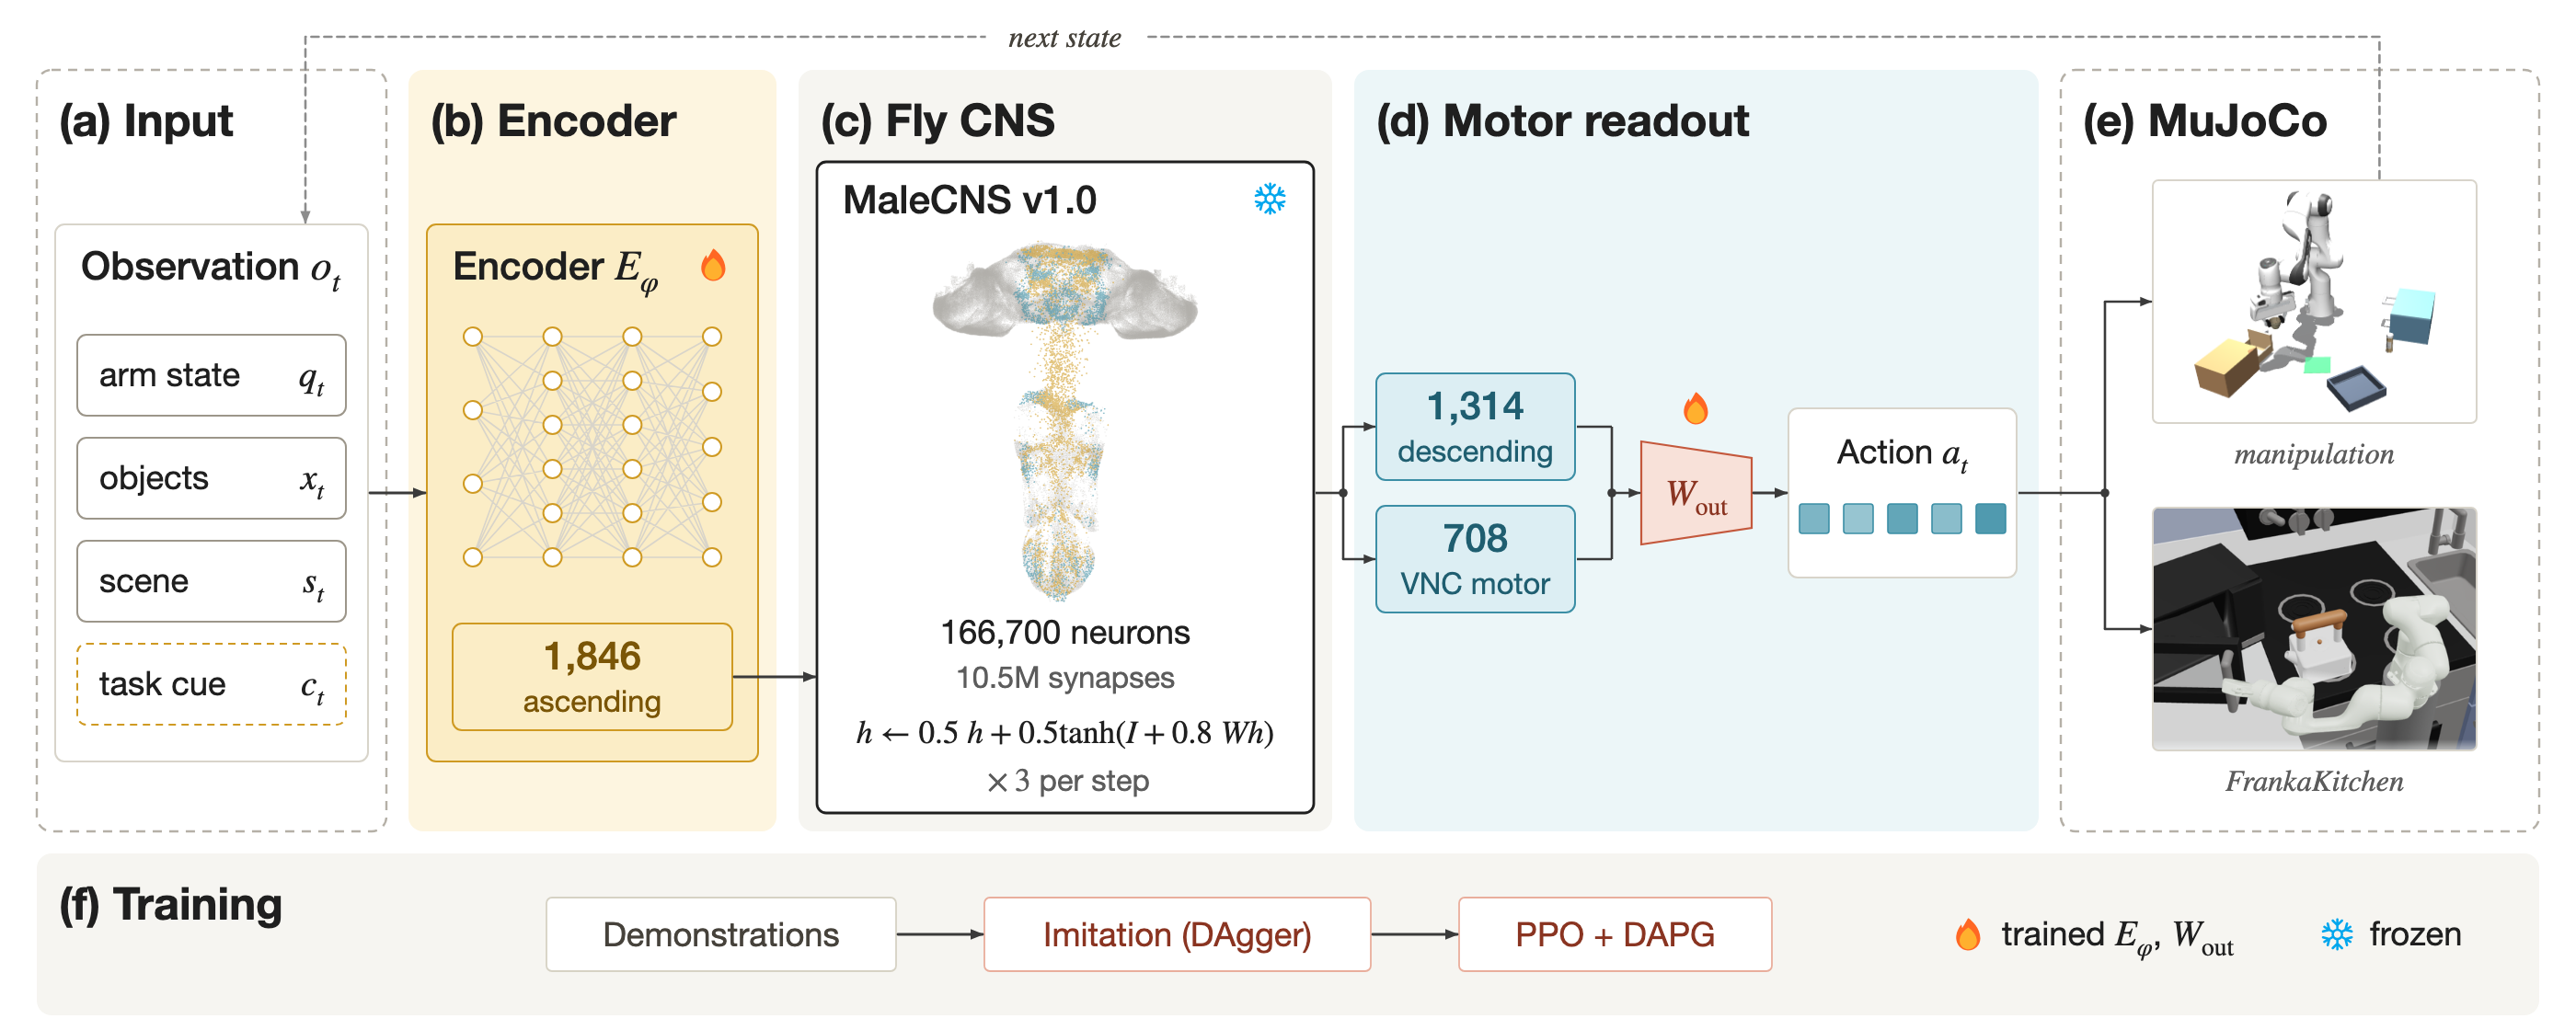
\includegraphics[width=\textwidth]{pipeline-figure.png}
\caption{One control step of FlyArm.
(a) The observation is simulator state: arm $q_t$, objects $x_t$, scene $s_t$ and, on the manipulation benchmark, a task cue $c_t$.
(b) The trained encoder $E_\phi$ writes currents into the 1,846 ascending neurons only.
(c) The MaleCNS v1.0 connectome is frozen; each control step runs three steps of $h \leftarrow 0.5h + 0.5\tanh(I + 0.8Wh)$ on all 166,700 neurons.
The soma map shows measured soma locations (gray), the declared inputs (amber) and outputs (teal).
(d) The 1,314 descending and 708 VNC motor neurons pass a fixed readout normalization and the trained linear decoder $W_{\mathrm{out}}$ into the action $a_t$.
(e) MuJoCo executes the action; the renders are a frame of a connectome controller on a test episode and the FrankaKitchen scene.
(f) Only $E_\phi$ and $W_{\mathrm{out}}$ are trained, by imitation and then PPO with DAPG.}
\label{fig:pipeline}
\end{figure*}

\section{Controller}
\label{sec:method}

\paragraph{Connectome.}
We compile the MaleCNS v1.0 release into a sparse matrix over its 166,700 annotated neurons.
A connection is kept when two neurons share at least three synaptic contacts (10,520,377 pairs, 104 million synapses, 84\% of all synapses between annotated neurons); its sign is $+1$ for acetylcholine, $-1$ for GABA and glutamate and $0$ for other or unclear transmitters, and each neuron's incoming absolute strength is normalized to at most one.
The pack is hash-pinned and a run refuses any other pack.

\paragraph{Dynamics.}
The network state $h \in \mathbb{R}^{166{,}700}$ follows a leaky rate model,
\begin{equation}
h \leftarrow \tfrac{1}{2} h + \tfrac{1}{2}\tanh\!\left(I + g\,W h\right), \qquad g = 0.8,
\end{equation}
with three neural steps per control step at 20\,Hz; the readout is the mean of the output rates over the three steps, and the state persists across control steps within an episode.
The recurrence runs in MLX \citep{mlx2023} with a custom Metal sparse kernel, about 4\,ms per control step on an Apple laptop GPU.

\paragraph{Interface.}
Input and output neurons are chosen by the official \texttt{superclass} annotation, not by hand: the input current $I$ is non-zero only on the 1,846 \texttt{ascending\_neuron} cells, and the decoder reads only the 1,314 \texttt{descending\_neuron} and 708 \texttt{vnc\_motor} cells.
The two sets are disjoint, so with every connectome edge removed the output is exactly zero for any input: the connectome is the only channel from observation to action.
On the manipulation benchmark the encoder $E_\phi$ is a two-layer tanh MLP of width 256 from the 300 observation features (below) to the 1,846 input currents; on FrankaKitchen it is linear.
Before the decoder, output rates are centred and scaled to unit expected norm with constants computed once from demonstrations and then frozen; without this, the first Adam updates on 2,022 correlated outputs saturate the decoder.
The decoder $W_{\mathrm{out}}$ is linear with a $\tanh$.
On the manipulation benchmark the controller has 0.63 M trainable parameters (0.62 M in the encoder, 10 k in the decoder); the connectome has 10.5 M fixed weights.

\paragraph{Observation and action.}
On the manipulation benchmark the observation is 230 values of simulator state: the arm (21), four object slots of 22 values (position, offset from the hand, rotation, shape descriptor, grasp flag), the furniture (46) and a memoryless task cue (75) that names the current subgoal's skill, object and receptacle, the relevant offsets, and a 10-way motor phase computed from geometric predicates of the scene (aligned, at height, grasped, above the target); the reported controller receives the motor phase as zeros (Section~\ref{sec:results}).
Joint and object velocities are zeroed, because controllers cloned from states with velocities learned to keep doing what the velocities say.
Seventy fixed copies of the hand-relative offsets and heading errors, $\tanh(\delta/\sigma)$ at $\sigma$ of one and four control steps, let the encoder resolve the millimetres that decide between hovering and descending.
The action is an end-effector step $(\Delta x, \Delta y, \Delta z, \Delta\psi, g)$ in $[-1,1]$, at most 14\,mm and 0.05\,rad per step, executed by damped least-squares inverse kinematics on the Menagerie Panda \citep{menagerie2022} in MuJoCo \citep{todorov2012mujoco} over 25 physics steps of 2\,ms.
On FrankaKitchen the observation is the benchmark's 30 position features and the action its 9 joint-velocity commands.

\section{Training}
\label{sec:training}

\begin{figure*}[t]
\centering
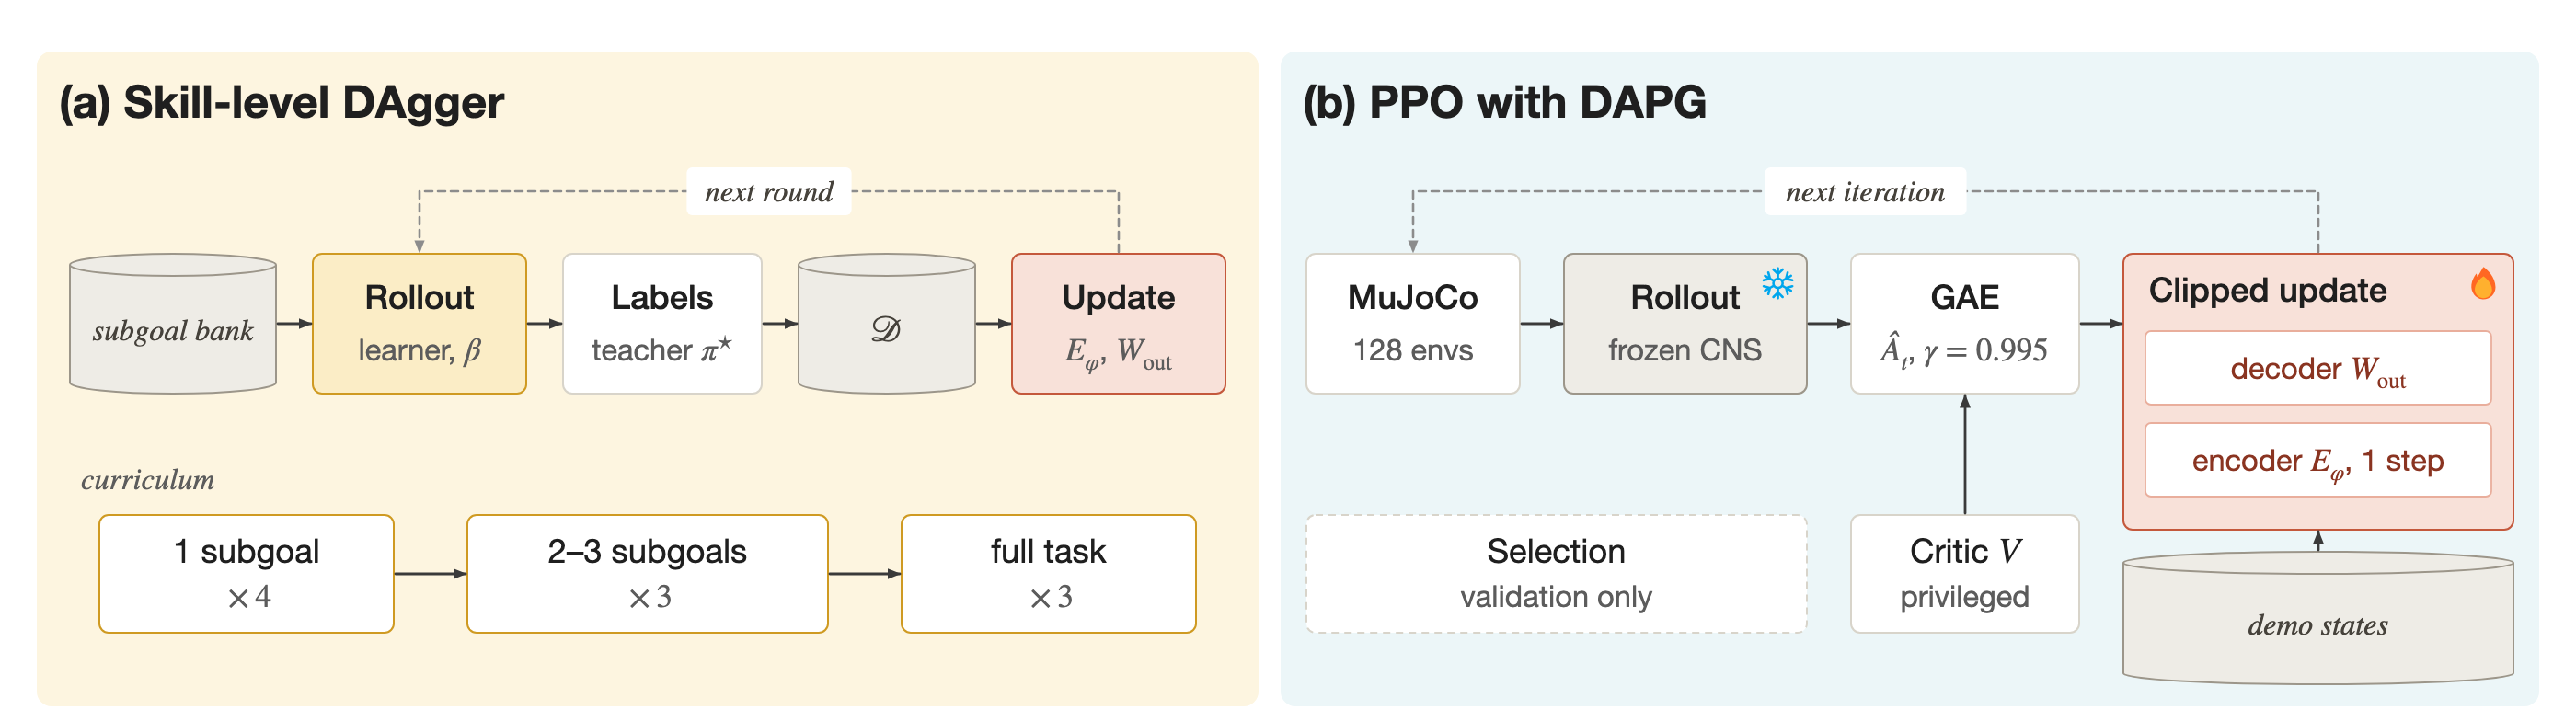
\includegraphics[width=\textwidth]{training-figure.png}
\caption{Training on the manipulation benchmark.
(a) Skill-level DAgger: each round resets 256 batched episodes to recorded subgoal starts or true starts, rolls out the learner (mixed with the teacher with probability $\beta$ in the first two rounds), labels every visited state with the privileged scripted teacher $\pi^\star$, aggregates the labels in $\mathcal{D}$, and updates $E_\phi$ and $W_{\mathrm{out}}$ by truncated backpropagation through the frozen connectome; the curriculum runs four rounds of single subgoals, three of two to three subgoals and three of full tasks.
(b) PPO with DAPG: 128 batched environments, rollouts through the frozen connectome, a critic on privileged state and GAE, clipped updates for the decoder and for the encoder through one control step, demonstration terms for both from states replayed through the current encoder every 25 iterations, and checkpoint selection on validation episodes only.}
\label{fig:training}
\end{figure*}

\paragraph{Imitation.}
The teacher on the manipulation benchmark is a scripted controller with privileged state that re-derives its phase from the scene whenever the current subgoal changes, so it can label any state a learner reaches.
Plain behaviour cloning and task-level DAgger \citep{ross2011dagger} both failed on full tasks: the learner stalled early and never produced the states of later subgoals.
Skill-level DAgger (Figure~\ref{fig:training}a) instead resets episodes to recorded starts of individual subgoals, so every skill is practised from its own start distribution from the first round.
Each round collects 256 episodes, labels every state with the teacher, and trains on the aggregate with an L1 loss over windows of 16 control steps after a burn-in of 16 steps of neural state, with skill-balanced weights capped at five.
After ten rounds the aggregate holds 1.8 M labelled steps; the checkpoint is selected on train-split validation episodes.
On FrankaKitchen, imitation is DAgger with a tracker of the benchmark's demonstrations.

\paragraph{PPO with a demonstration term.}
We fine-tune with PPO \citep{schulman2017ppo} and GAE \citep{schulman2016gae} ($\gamma = 0.995$, $\lambda = 0.95$, clip 0.2) on 128 batched environments with rollouts of 64 steps, a critic on privileged state that is warmed up for 50 iterations before the policy moves, and advantages clipped at ten standard deviations.
Every policy update adds the DAPG term \citep{rajeswaran2018dapg}, the squared error to the teacher's action on a minibatch of 1,024 demonstration steps, with weight one.
The reward pays a bonus of 50 per subgoal in task order, potential-based shaping toward the current subgoal (weight 10), a potential on the displacement of objects the task does not involve (weight 5), and small penalties for stray robot contact and large actions; every level term is a penalty, so stalling is never worth more than finishing.
Training runs on a curriculum of two to three subgoals from subgoal resets and then full tasks, with subgoal resets drawn from a bank recorded by the teacher.

\paragraph{Training the encoder with PPO.}
With the encoder frozen, PPO tunes only the 10 k decoder weights.
We also update the encoder, with the gradient truncated to one control step: the connectome state before the step is a constant, and only that step's three neural updates are differentiated, so a single step's graph is alive at a time.
The encoder's loss is PPO's clipped surrogate on the rollout's log-probabilities plus its own DAPG term, differentiated through the same single step from connectome states stored before 1,024 demonstration steps.
Every 25 iterations the demonstrations are replayed through the current encoder, so the decoder's DAPG features and the stored states follow the encoder.
An unclipped encoder update collapsed the policy twice in one run (validation 41 of 56 at iteration 100, then 5 of 56 at 250 and 0 of 56 at 400); with the clipped surrogate and a learning rate of $10^{-5}$ the run was stable over 400 iterations.

\paragraph{Selection and evaluation.}
Checkpoints are selected only on validation episodes of the train split.
Final numbers use 32 fresh episodes per task template on every test split, from seed blocks disjoint from every episode used for training or selection, with deterministic actions and Wilson 95\% intervals \citep{wilson1927}.
For the three training seeds and the shuffled-connectome control the protocol was fixed before any of their results: the imitation checkpoint is the round among 7, 8 and 9, and the PPO checkpoint the iteration among 150, 300 and 500, with the most successes on 112 validation episodes (ties to the later one); nothing else differs between seeds or between the measured and the shuffled graph.
Across seeds we report the mean and range of the success rate and the pooled count; the measured and the shuffled connectome are compared by Welch's $t$-test on the seed-level rates and by Fisher's exact test on pooled episodes, and paired conditions on the same episodes by exact McNemar tests.
Applied to seed 0, which was trained before the protocol was written, the protocol selects the checkpoints already reported.

\section{Benchmarks}

\paragraph{FrankaKitchen.}
We use the official Gymnasium-Robotics FrankaKitchen environment and the kitchen-complete task of D4RL \citep{fu2020d4rl}: open the microwave, move the kettle, flip the light switch and slide the cabinet, in that order.
Flat reinforcement learning fails on it \citep{gupta2019relay}.
We report the benchmark score (tasks ever completed at the threshold 0.3) from the benchmark start and from starts whose joints are perturbed by 0.2 and 0.3\,rad, which were never used in training, and a strict score counting elements that end within 0.1 of their goal.

\begin{figure*}[t]
\centering
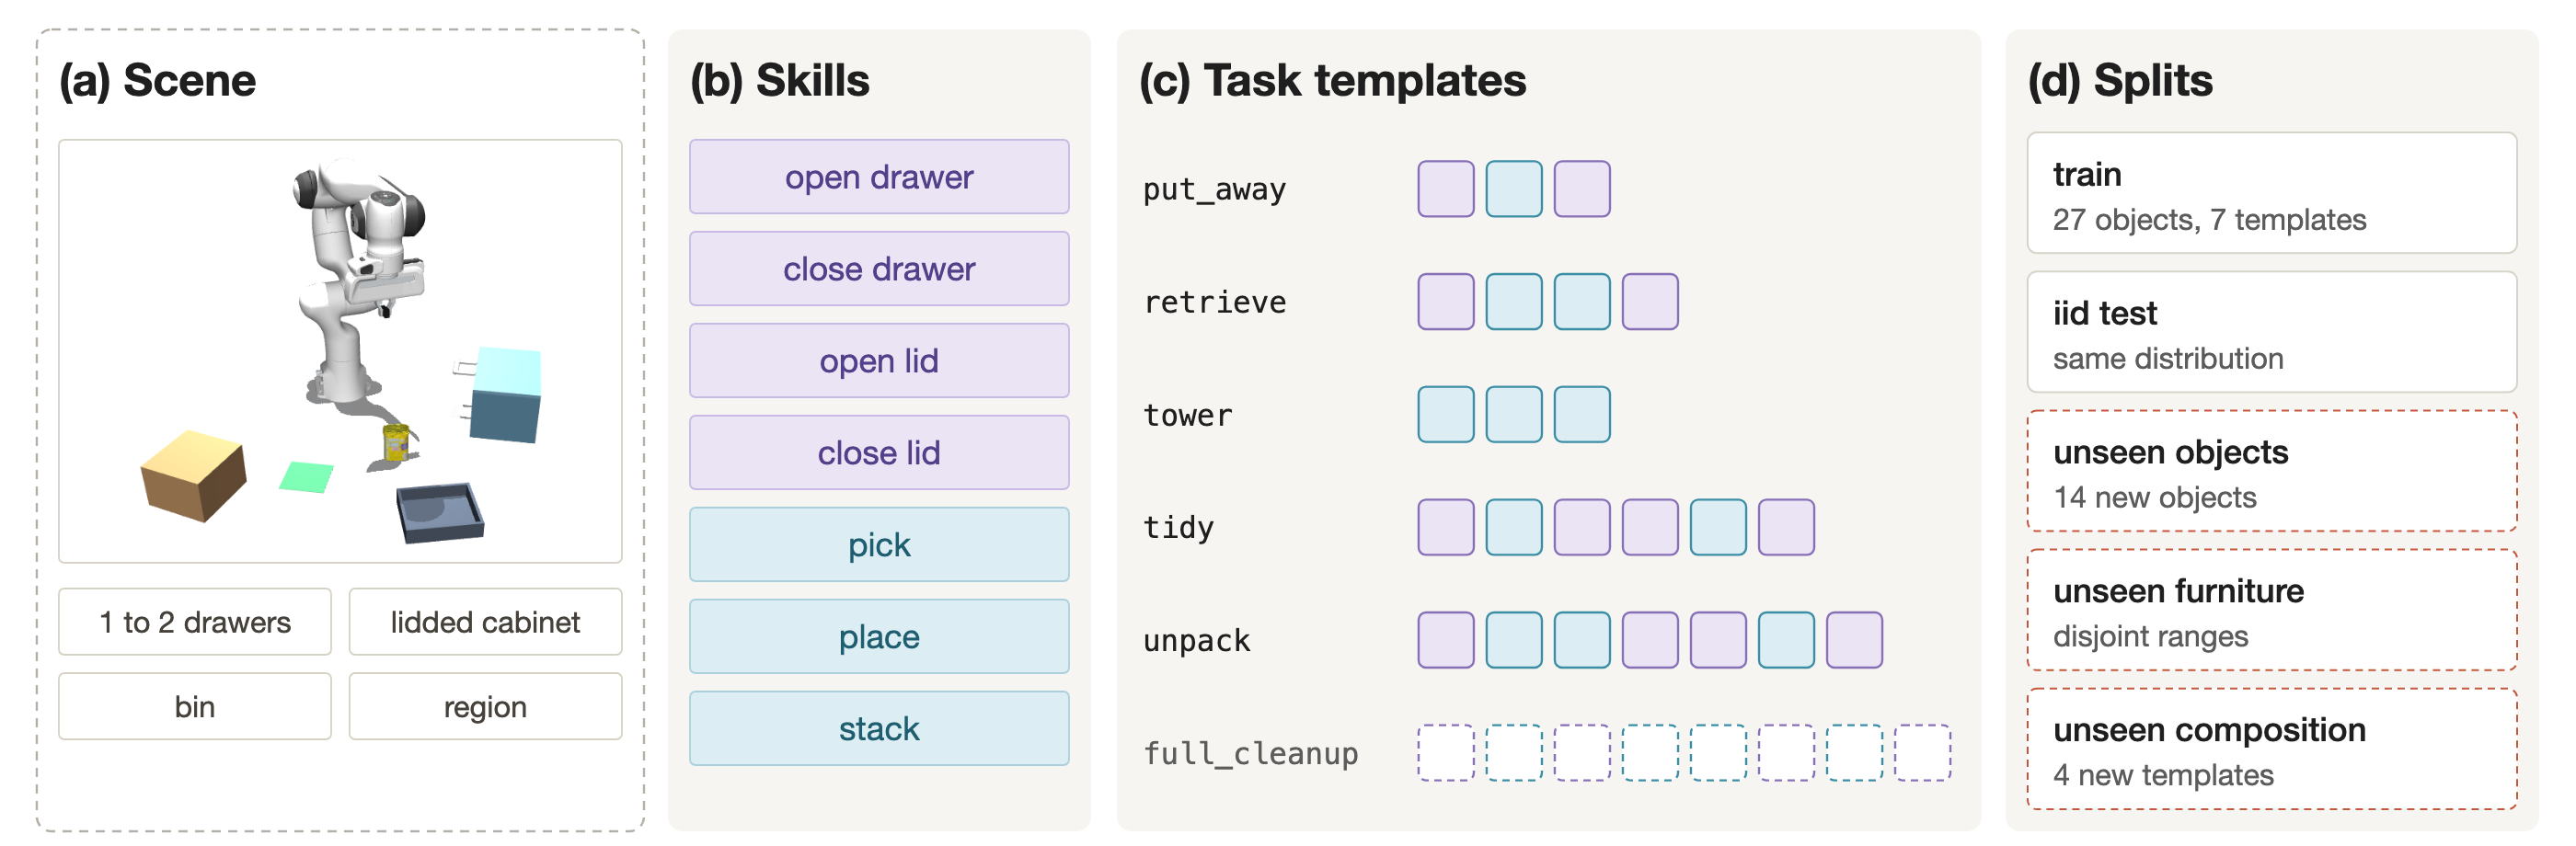
\includegraphics[width=\textwidth]{benchmark-figure.png}
\caption{The articulated multi-step manipulation benchmark.
(a) A real render of a reset: a drawer cabinet with one or two drawers, a cabinet with a hinged lid over a shelf, a bin and a marked region, with two to four scanned household objects.
(b) Seven skills with physical success checks: articulations (purple) and object skills (blue).
(c) Task templates as sequences of skills; the four held-out compositions (here \texttt{full\_cleanup}, dashed) contain adjacent pairs of steps that no training template has.
(d) Five preregistered splits; red dashed splits hold out objects, furniture ranges or task orders.}
\label{fig:benchmark}
\end{figure*}

\paragraph{Articulated multi-step manipulation.}
The Panda works a tabletop kitchen (Figure~\ref{fig:benchmark}): it pulls drawers open and pushes them shut, lifts a cabinet lid, and puts 41 scanned household objects into drawers, onto the shelf, into the bin or onto the region, or stacks them into towers.
Each skill has a strict physical check; placing, for example, requires 128 support points of the object's collision hull inside the receptacle, no robot contact, and ten consecutive steps at rest.
Seven training templates have three to seven subgoals, and four held-out compositions have five to eight; the horizon is 200 plus 300 control steps per subgoal (1,100 to 2,600 steps).
Progress is derived from the scene every step, so undoing a subgoal makes it current again.
Five splits are preregistered and checked against the code: train, an iid test split, unseen objects (the 14 held-out objects of a separate grasp catalogue), unseen furniture (every layout factor from a range disjoint from training) and unseen composition.
All furniture is built from MuJoCo primitives and resized per episode through per-simulation model fields, so 128 episodes step in parallel.
The privileged teacher solves 111 of 112 iid test episodes, 111 of 112 with unseen objects, 110 of 112 with unseen furniture and 61 of 64 unseen compositions.

\section{Results}
\label{sec:results}

\paragraph{FrankaKitchen.}
Table~\ref{tab:kitchen} reports the official environment over 50 test episodes per condition.
The four-task controller completes all four tasks in every episode, including from perturbed starts it never trained on; the published behaviour-cloning result on kitchen-complete is about 65 \citep{fu2020d4rl}.
Blind replay of a demonstration from the perturbed starts scores 16 to 19, so the scores measure closed-loop control.
The motion-quality controller adds penalties for stray contact, for disturbing other objects and for large and abrupt commands, holds half of each bonus until the element is within 0.1 of its goal, and raises the strict score from 50 to about 70 at a small cost in the benchmark score from perturbed starts.
The four-task stage replicates on three PPO seeds (100.0, 100.0 and 97.5 over 20 perturbed test episodes in the batched environment).

\begin{table}[t]
\centering
\small
\caption{FrankaKitchen, official environment, 50 test episodes per condition. Score: tasks completed at the benchmark threshold, times 25. Strict: elements within 0.1 of their goal at the end.}
\label{tab:kitchen}
\begin{tabular}{@{}llrrr@{}}
\toprule
Controller & Start & Score & All four & Strict \\
\midrule
\multirow{3}{*}{Four-task} & benchmark & 100.0 & 50/50 & 50.0 \\
 & 0.2\,rad & 100.0 & 50/50 & 50.0 \\
 & 0.3\,rad & 100.0 & 50/50 & 50.0 \\
\midrule
\multirow{3}{*}{Motion quality} & benchmark & 100.0 & 50/50 & 69.5 \\
 & 0.2\,rad & 97.5 & 48/50 & 70.5 \\
 & 0.3\,rad & 96.5 & 46/50 & 68.0 \\
\bottomrule
\end{tabular}
\end{table}

\paragraph{Articulated manipulation.}
Table~\ref{tab:manip} compares the stages of the recipe on the same fresh test episodes, with and without the motor-phase cue.
With the cue, PPO on the decoder alone adds 4 to 6 points to imitation, and training the encoder as well adds another 13 points on held-in test episodes and 22 points with unseen objects (episode-level Fisher exact tests against decoder-only PPO: $p = 0.005$ and $p = 2\times10^{-6}$).
Without the cue, so that the phase has to come from the rest of the observation and the connectome's recurrent state, the same recipe is at least as good on every split: 76.3\% on held-in test episodes and 82.6\% with unseen objects against 69.6\% and 75.0\% with the cue ($p = 0.14$ and $0.064$), and identical counts on unseen furniture and compositions.
We therefore report the controller without the phase cue.
On unseen furniture and unseen compositions all stages differ little.
The reported controller completes 86\% of the subgoals of iid episodes and 89\% with unseen objects.

\begin{table}[t]
\centering
\small
\caption{Articulated manipulation: full-task success (\%) from true starts, 32 fresh episodes per template (224 per split, 128 for the four held-out compositions). Reported controller (bold) with Wilson 95\% intervals: iid 70--81, unseen objects 77--87, unseen furniture 31--43, held-out compositions 20--35. One training seed each.}
\label{tab:manip}
\setlength{\tabcolsep}{3.5pt}
\begin{tabular}{@{}lrrrr@{}}
\toprule
Controller & iid & objects & furniture & comp. \\
\midrule
\multicolumn{5}{@{}l}{\emph{with the motor-phase cue}} \\
Imitation & 51.3 & 49.6 & 27.2 & 18.8 \\
+ PPO, decoder & 56.3 & 53.1 & 32.1 & 25.0 \\
+ PPO, enc.\ and dec. & 69.6 & 75.0 & 36.6 & 26.6 \\
\midrule
\multicolumn{5}{@{}l}{\emph{without the motor-phase cue}} \\
Imitation & 63.4 & 64.7 & 28.1 & 17.2 \\
+ PPO, enc.\ and dec. & \textbf{76.3} & \textbf{82.6} & \textbf{36.6} & \textbf{26.6} \\
\bottomrule
\end{tabular}
\end{table}

\paragraph{Lesions of the trained controller.}
To see which parts of the frozen connectome the trained controller uses, we lesion it at test time without retraining (Figure~\ref{fig:lesions}): a group of non-interface neurons is clamped to zero after every neural step, and each anatomical group is compared with two random sets of the same size drawn from all non-interface neurons, on the same 112 iid test episodes (exact McNemar tests).
Clearing the recurrent state before every control step, while keeping the three neural steps within it, removes every success (0 of 112): the controller depends on the connectome's state carried across control steps.
The effect of silencing follows the anatomy rather than the number of neurons silenced.
Silencing the 13,161 VNC interneurons, which relay descending neurons to motor neurons, lowers success from 87 to 46 of 112, while random sets of the same size leave 84 and 79 (paired against each random set, $p = 2\times10^{-9}$ and $10^{-6}$).
Silencing the 99,167 optic-lobe neurons, which receive no input in this task, leaves 94, while random sets of that size leave 39 and 1.
The central brain (82 against 75 and 75) and the sensory neurons (78 against 82 and 76) do not differ from their random sets.
With every non-interface neuron silenced, only the interface neurons and the edges among them remain; 16 of 112 episodes still succeed, which bounds what the direct ascending-to-output edges carry (16\% of the incoming weight of descending neurons and 5\% of motor neurons).
A partial random lesion of 99,167 neurons does worse than this clean removal, so a lesion can also derail the trained readout rather than only remove capacity; the lesions are of one trained controller.

\begin{figure}[t]
\centering
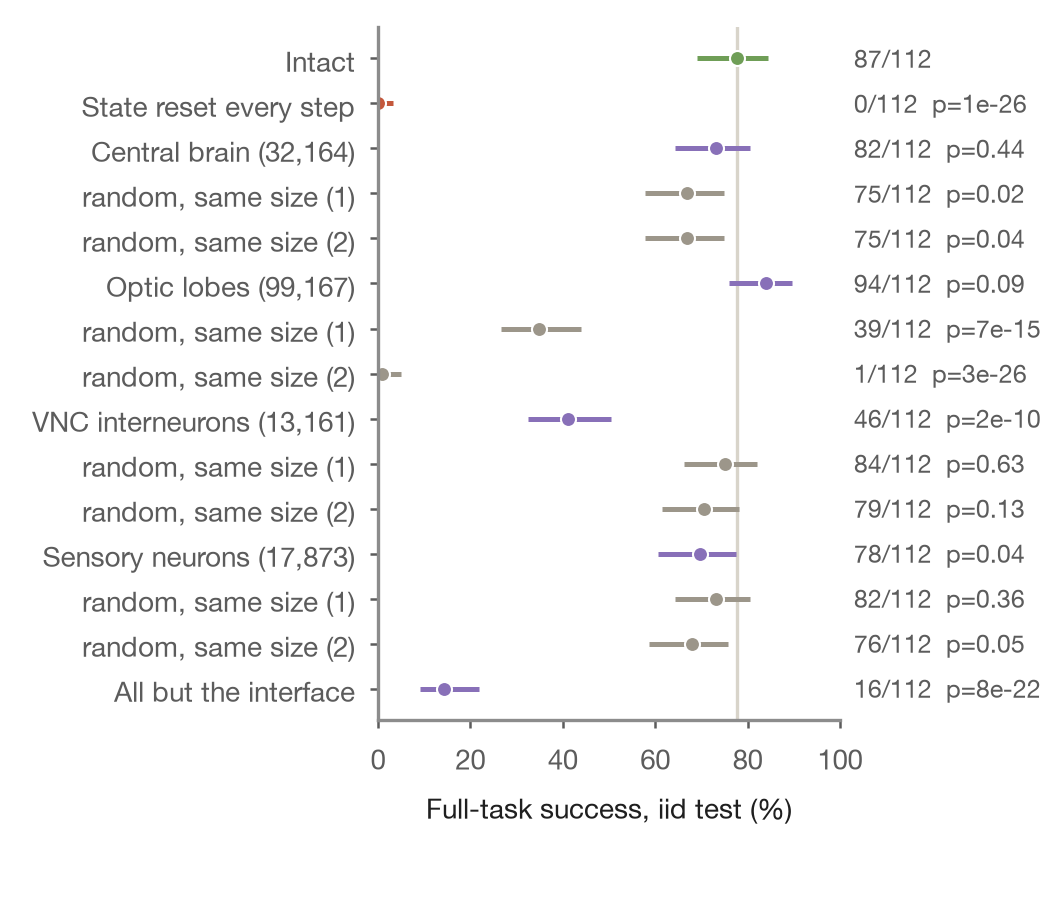
\includegraphics[width=\columnwidth]{lesion-figure.png}
\caption{Test-time lesions of the reported controller on 112 iid test episodes: full-task success with Wilson 95\% intervals and the number of successful episodes; the dashed line is intact. (a) The recurrent state cleared before every control step, and only the interface neurons left. (b) Each anatomical group silenced (purple; schematic of the fly CNS with the group filled) between two random non-interface sets of the same size (grey). Brackets: exact McNemar $p$ on the same episodes, against intact in (a) and of the anatomical lesion against each random set in (b).}
\label{fig:lesions}
\end{figure}

\paragraph{Where it fails.}
A failure analysis of the decoder-only PPO controller on 16 fresh episodes per template found nearly every failure to be the learner's (the teacher solves the same episodes): of 218 failed episodes, 151 stopped at a placement, most often on the shelf (44) and in the region (29), then at stacking (10) and closing a drawer (8).
Placing into a drawer is solved (16 of 16 on every split), while \texttt{retrieve\_to\_shelf}, a held-out composition, stops at opening the drawer in 16 of 16 episodes.
On unseen furniture the controller reaches handles and receptacles at positions outside the training ranges less reliably, which a state-based encoder trained on 1.8 M steps of seen layouts does not extrapolate to.

\paragraph{What did not help.}
Several changes that were expected to help did not (Table~\ref{tab:negative}).
Weighting subgoal resets towards the failing placements raised in-run validation but not the 112-episode validation set, both in imitation and in PPO.
A readout gated by the observable skill and motor phase, one decoder per program, was motivated by the finding that the teacher is close to linear within a skill and phase (L1 0.068 per skill and phase against 0.258 for one linear map from the observation) but fitted the teacher no better than the single decoder, which already reads out of a trained nonlinear encoder and the connectome, and generalized worse to unseen furniture (5 of 56 against 15 of 56).
Separate decoders per program also took full-size Adam steps on rarely visited programs; a shared decoder with slow per-program corrections fixed the instability but not the generalization.

\begin{table}[t]
\centering
\small
\caption{Changes that did not improve the controller: successes on the 112-episode validation set (16 per template). Rows marked $^\dagger$ were scored before the change to capsule rods (Section~\ref{sec:results}), which moves scores by one or two episodes.}
\label{tab:negative}
\begin{tabular}{@{}lr@{}}
\toprule
Controller & Validation \\
\midrule
Imitation, selected round & 64/112 \\
\quad + failure-targeted resets, best round$^\dagger$ & 64/112 \\
\quad + gated readout, best round & 63/112 \\
PPO, decoder only & 75/112 \\
\quad + failure-targeted resets$^\dagger$ & 73/112 \\
PPO, encoder and decoder, unclipped & 83/112 \\
PPO, encoder and decoder, clipped & 86/112 \\
\quad without the phase cue (reported) & \textbf{89/112} \\
\bottomrule
\end{tabular}
\end{table}

\paragraph{A simulator failure.}
Two training runs died without an error message.
Crash reports showed segmentation faults inside MuJoCo 3.13's native convex collision (EPA) at the same state twice: a finger pad, a box, pressed 7.9\,mm into the lid's handle bar, a cylinder, a pair with no analytic collider.
Raising the collision iteration cap only moved the failure; every furniture rod is now a capsule of the same end-to-end length, whose collider against a box is analytic, which changed validation scores by one or two episodes in 112.

\section{Controls, limitations and next steps}
\label{sec:limits}

\paragraph{Controls.}
The claim of this report is that a frozen whole-CNS connectome can be trained to control the arm on these tasks.
Whether its measured wiring matters is a separate claim.
The lesions above show that the trained controller depends on specific anatomical groups rather than on the number of neurons, but not that the measured wiring trains better than another graph; that needs controls run through the identical pipeline with several seeds: a degree-preserving shuffle of the connectome (running, three seeds) and parameter-matched GRU and MLP controllers.
So far only their imitation stage exists on the manipulation benchmark, with one seed each: on iid validation the measured connectome reaches 51.8\%, its shuffle 44.6\%, a matched GRU 66.1\% and a matched MLP 26.8\%; the episode-level difference between the measured wiring and its shuffle, pooled over splits, has $p = 0.016$, but seed-level statistics are required before it is a claim, and the GRU, which trains its own recurrence, is ahead.
In an earlier real-contact pick-and-place task the complete connectome lifted 58 of 72 test cubes against 27 for its shuffle and 33 for a matched GRU over three training seeds, and resetting the neural state every step removed lifting entirely, but that task and interface are superseded here.

\paragraph{Limitations.}
Observations are simulator state, not vision, and on the manipulation benchmark the task cue (the current subgoal's skill, object, receptacle and target) comes from the task plan and the simulator state, so the task's order is given to the controller rather than inferred; the motor phase within a skill is not given.
The rate model is an abstraction on the measured wiring, not a physiological or spiking emulation.
All results are in simulation, and the manipulation results are one training seed so far.

\paragraph{Next steps.}
Seeds and controls for the reported controller; a weaker task cue that names only the goal; perception from rendered images through a privileged-teacher-to-student distillation; and transfer to public benchmarks.

\section*{Reproducibility}
Code, configurations, the research log with every experiment including failed ones, and all result files are in the repository.
The connectome pack is rebuilt from hash-pinned official exports and fingerprinted.
Every figure in this report is generated by a script in \texttt{docs/figures/src}.

\appendix
\section{Hyperparameters and compute}
\label{app:hyper}

Table~\ref{tab:hyper} lists the settings of the reported manipulation controller; the configuration files in \texttt{configs/} are authoritative.
One run of the full recipe takes about 8.5\,h of skill-level DAgger and 6.3\,h of PPO on one Apple M5 Max (64\,GB unified memory); the final evaluation of one checkpoint (800 episodes) takes about 17 minutes.
No hyperparameter was tuned on test episodes.

\begin{table*}[t]
\centering
\small
\caption{Settings of the reported manipulation controller.}
\label{tab:hyper}
\begin{tabular}{@{}ll@{}}
\toprule
\multicolumn{2}{@{}l}{\emph{Controller}} \\
Rate model & $\alpha = 0.5$, $g = 0.8$, 3 neural steps per control step \\
Encoder & MLP $300 \to 256 \to 256 \to 1{,}846$, tanh \\
Decoder & linear $2{,}022 \to 5$, tanh, unit-norm readout \\
Trainable parameters & 627,385 \\
\midrule
\multicolumn{2}{@{}l}{\emph{Skill-level DAgger}} \\
Rounds & 4 single subgoal, 3 two to three, 3 full tasks \\
Episodes per round & 256 (teacher mixing $\beta$ 0.5, 0.25, then 0) \\
Updates & 3,000 in round 0, then 10 epochs, at most 3,000 \\
Loss, optimizer & L1, Adam, learning rate $10^{-3}$ \\
Windows & 64 of 16 steps after a 16-step burn-in \\
Skill weights & balanced, capped at 5 \\
\midrule
\multicolumn{2}{@{}l}{\emph{PPO with DAPG}} \\
Environments, rollout & 128, 64 steps \\
Iterations & 200 two to three subgoals, 300 full tasks \\
Epochs, minibatch & 4, 2,048 \\
$\gamma$, $\lambda$, clip & 0.995, 0.95, 0.2 \\
Learning rates & decoder $3\times10^{-4}$, encoder $10^{-5}$, critic $10^{-3}$ \\
Exploration & $\log\sigma = -1.2$ \\
DAPG & weight 1, minibatch 1,024, 60,000 steps, refresh every 25 \\
Reward & subgoal 50, shaping 10, disturbance 5, contact 0.05, action 0.01 \\
\bottomrule
\end{tabular}
\end{table*}

\bibliographystyle{plainnat}
\bibliography{refs}

\end{document}
